\documentclass[a4paper,12pt]{jarticle}

% レイアウト
\setlength{\hoffset}{0cm}
\setlength{\oddsidemargin}{-3mm}
\setlength{\evensidemargin}{-3cm}
\setlength{\marginparsep}{0cm}
\setlength{\marginparwidth}{0cm}
\setlength{\textheight}{24.7cm}
\setlength{\textwidth}{17cm}
\setlength{\topmargin}{-45pt}


\renewcommand{\baselinestretch}{1.6}
\renewcommand{\floatpagefraction}{1}
\renewcommand{\topfraction}{1}
\renewcommand{\bottomfraction}{1}
\renewcommand{\textfraction}{0}
\renewcommand\thefootnote{\arabic{footnote})}

% パッケージ
\usepackage[dvipdfmx]{graphicx}
\usepackage{amsmath,amssymb,epsfig}
\usepackage{eucal}
\usepackage{bm}
\usepackage{ascmac}
\usepackage{pifont}
\usepackage{multirow}
\usepackage{enumerate}
\usepackage{cases}
\usepackage{type1cm}
\usepackage{cancel}
\usepackage{url}
\usepackage{cite}
%\usepackage{color}
\usepackage[dvipdfmx]{color}
\usepackage{caption}
\usepackage[caption=false]{subfig}
\captionsetup[figure]{labelsep=space}
\usepackage{url}
\usepackage{here}

% 擬似コード作成用
\usepackage[ruled,vlined]{algorithm2e}
\usepackage{setspace}
\DeclareRelationFont{JY1}{mc}{it}{}{OT1}{cmr}{it}{}
\DeclareRelationFont{JT1}{mc}{it}{}{OT1}{cmr}{it}{}
\DeclareFontShape{JY1}{mc}{m}{it}{<5> <6> <7> <8> <9> <10> sgen*min
    <10.95><12><14.4><17.28><20.74><24.88> min10
    <-> min10}{}
\DeclareFontShape{JT1}{mc}{m}{it}{<5> <6> <7> <8> <9> <10> sgen*tmin
    <10.95><12><14.4><17.28><20.74><24.88> tmin10
    <-> tmin10}{}
\DeclareRelationFont{JY1}{mc}{sl}{}{OT1}{cmr}{sl}{}
\DeclareRelationFont{JT1}{mc}{sl}{}{OT1}{cmr}{sl}{}
\DeclareFontShape{JY1}{mc}{m}{sl}{<5> <6> <7> <8> <9> <10> sgen*min
    <10.95><12><14.4><17.28><20.74><24.88> min10
    <-> min10}{}
\DeclareFontShape{JT1}{mc}{m}{sl}{<5> <6> <7> <8> <9> <10> sgen*tmin
    <10.95><12><14.4><17.28><20.74><24.88> tmin10
    <-> tmin10}{}
\DeclareRelationFont{JY1}{mc}{sc}{}{OT1}{cmr}{sc}{}
\DeclareRelationFont{JT1}{mc}{sc}{}{OT1}{cmr}{sc}{}
\DeclareFontShape{JY1}{mc}{m}{sc}{<5> <6> <7> <8> <9> <10> sgen*min
    <10.95><12><14.4><17.28><20.74><24.88> min10
    <-> min10}{}
\DeclareFontShape{JT1}{mc}{m}{sc}{<5> <6> <7> <8> <9> <10> sgen*tmin
    <10.95><12><14.4><17.28><20.74><24.88> tmin10
    <-> tmin10}{}
\DeclareRelationFont{JY1}{gt}{it}{}{OT1}{cmbx}{it}{}
\DeclareRelationFont{JT1}{gt}{it}{}{OT1}{cmbx}{it}{}
\DeclareFontShape{JY1}{mc}{bx}{it}{<5> <6> <7> <8> <9> <10> sgen*goth
    <10.95><12><14.4><17.28><20.74><24.88> goth10
    <-> goth10}{}
\DeclareFontShape{JT1}{mc}{bx}{it}{<5> <6> <7> <8> <9> <10> sgen*tgoth
    <10.95><12><14.4><17.28><20.74><24.88> tgoth10
    <-> tgoth10}{}
\DeclareRelationFont{JY1}{gt}{sl}{}{OT1}{cmbx}{sl}{}
\DeclareRelationFont{JT1}{gt}{sl}{}{OT1}{cmbx}{sl}{}
\DeclareFontShape{JY1}{mc}{bx}{sl}{<5> <6> <7> <8> <9> <10> sgen*goth
    <10.95><12><14.4><17.28><20.74><24.88> goth10
    <-> goth10}{}
\DeclareFontShape{JT1}{mc}{bx}{sl}{<5> <6> <7> <8> <9> <10> sgen*tgoth
    <10.95><12><14.4><17.28><20.74><24.88> tgoth10
    <-> tgoth10}{}
\DeclareRelationFont{JY1}{gt}{sc}{}{OT1}{cmbx}{sc}{}
\DeclareRelationFont{JT1}{gt}{sc}{}{OT1}{cmbx}{sc}{}
\DeclareFontShape{JY1}{mc}{bx}{sc}{<5> <6> <7> <8> <9> <10> sgen*goth
    <10.95><12><14.4><17.28><20.74><24.88> goth10
    <-> goth10}{}
\DeclareFontShape{JT1}{mc}{bx}{sc}{<5> <6> <7> <8> <9> <10> sgen*tgoth
    <10.95><12><14.4><17.28><20.74><24.88> tgoth10
    <-> tgoth10}{}
\DeclareRelationFont{JY1}{gt}{it}{}{OT1}{cmr}{it}{}
\DeclareRelationFont{JT1}{gt}{it}{}{OT1}{cmr}{it}{}
\DeclareFontShape{JY1}{gt}{m}{it}{<5> <6> <7> <8> <9> <10> sgen*goth
    <10.95><12><14.4><17.28><20.74><24.88> goth10
    <-> goth10}{}
\DeclareFontShape{JT1}{gt}{m}{it}{<5> <6> <7> <8> <9> <10> sgen*tgoth
    <10.95><12><14.4><17.28><20.74><24.88> tgoth10
    <-> tgoth10}{}
\endinput
%%%% end of jdummy.def

% カウンタの設定
\setcounter{section}{0}
\setcounter{subsection}{0}
\setcounter{subsubsection}{0}
\setcounter{equation}{0}

% キャプションの図をFigに変更
\renewcommand{\figurename}{Fig.}
\renewcommand{\tablename}{Tab.}

% 式番号を式(章番号.番号)に
\makeatletter
\renewcommand{\theequation}{\arabic{section}.\arabic{equation}}
\@addtoreset{equation}{section}
\makeatother

% 表紙
\title{\Large{電機システム制御特論\\ レポート課題3}
% {\large No title}
}
\author{\vspace{70mm}\\
九州工業大学\ \hspace{0mm} 工学府\\
機械知能工学専攻\ \hspace{0mm} 知能制御工学コース\\
\\
所属:\ 西田研究室\\
学籍番号:\ 17344219\\
提出者氏名:\ 二宮 \hspace{0mm} 悠二\\\vspace{5mm}\\}
\date{平成29年\ 5月\ 23日}

% ドキュメントの開始
\begin{document}
% 表紙
\titlepage
\maketitle
\thispagestyle{empty}
\newpage

% 目次
\thispagestyle{empty}
\tableofcontents
\newpage

% 課題内容
\section{課題内容}
%
次のシステムについて考える.
%
\begin{equation*}
 \begin{array}{c}
  \dot{x} = ax + bu + v \\
  y = x + w \\
 \end{array}
\end{equation*}
%
ただし,$ a = -0.02 , ~ b = 1.351 \times 10^{-3} $である.また,$ v $と$ w $は共に白色ガウス雑音であり,$ E \left\{v^2 \right\} = E \left\{w^2 \right\} = 0.7 $である.このとき,システム対するにカルマンフィルタを設計し,コンピュータシミュレーションによりその動作を示せ.


\section{カルマンフィルタ}
%
システムが実用される際に,そのパフォーマンスに影響を及ぼすような様々な雑音が存在する.
同一次元オブザーバはそれ自身が観測雑音に対していくつかのフィルタ機能を持つものの,観測信号にふくまれた雑音成分を取り除くには不十分であることが多い.確率システムに含まれるオブザーバゲインは与えられた雑音に対して最適化される可能性があるのだ.
これは雑音などの存在しない確定的な場合を対称としているためである.
それに対し,カルマンフィルタは確率的な枠組みで状態推定問題を検討しており,白色ガウス雑音のあるシステムの状態信号の最適な推定を行うことが可能である.{\bf Fig.}\ref{kalman}に制御系にカルマンフィルタを組み込んだ様子を示す.

また,本課題にて設計したのは連続時間でのカルマンフィルタである.これは,離散系からの拡張であるため,本稿では離散時間及び連続時間カルマンフィルタの原理について述べる.

% 状態方程式の状態を推定する方法として,ルーエンバーガによるオブザーバが有名であるが,これは雑音などの存在しない確定的な場合を対称としている.それに対し,カルマンフィルタは確率的な枠組みで状態推定問題を検討している.
%
\begin{figure}[tb]
 \begin{center}
  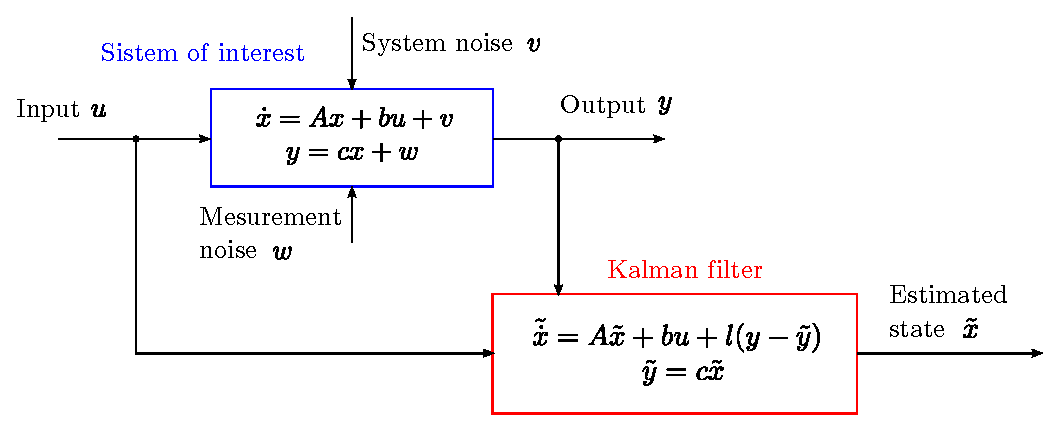
\includegraphics[scale=0.8]{../figure/eps/kalman.eps}
  \caption{カルマンフィルタを組み込んだ制御系}
  \label{kalman}
 \end{center}
\end{figure}
%


% \subsection{白色ガウス雑音}
% %
% 前述のカルマンフィルタの概要に出てきた白色ガウス雑音について説明する.

% 時系列$ y(k) $の分散が,

% まず,白色雑音とは,
% 平均値がゼロで,$ w(t) $と$ w(\tau) $ $ (t \neq \tau ) $が無相関であることを言う.
% 特に白色ノイズ線形要素を通過したときの出力が正規分布,あるいはガウス分布に従うとき,入力である白色雑音は白色ガウス雑音と呼ばれる.


\subsection{離散時間カルマンフィルタ}
%
未知パラメータ$ \mbox{\boldmath{$x$}} $がある離散系の状態方程式に従って変化している場合を考える.このとき,状態0から状態1への遷移が次の式で表されるものとする.
%
\begin{equation}
 x_1 = A_0 x_0 + B_0 w_0
\label{(1)}
\end{equation}
%
%ここで,$ \mbox{\boldmath{$A$}} $
%
ここで,$ A_0 $は離散系での$ (n \times n) $の推移行列,$ B_0 $は既知の$ (n \times r) $の行列である.ここで,$ w_0 $が系に加わる外乱ベクトルで,その平均が $ \bar{w}_0 $,共分散が$ Q_0 $であるとする.すなわち,
%
\begin{eqnarray}
 E(w_0) = \bar{w}_0 \\
 E[ ( w_0 - \bar{w}_0 )( w_0 - \bar{w}_0 )^T ] = Q_0
\end{eqnarray}
%
である.一方,状態量$ x_0 $についても同様に,平均が$ \hat{x}_0 $,共分散が$ P_o $であるとすると,
%
\begin{eqnarray}
 E(x_0) = \hat{x}_0 \\
 E[ ( x_0 - \hat{x}_0 )( x_0 - \hat{x}_0 )^T ] = P_0
\end{eqnarray}
%
を得る.さらに,$ x_0 $と$ w_0 $は無相関であるとすると,
%
\begin{equation}
 E(x_0 w_0) = 0
\end{equation}
%
が成り立つ.

以上より,状態1での平均値は次のようになる.
%
\begin{eqnarray}
 \bar{x}_1 = A_0 \hat{x}_0 + B_0 \bar{w}_0
\label{(7)}
\end{eqnarray}
%
さらに,(\ref{(1)}),(\ref{(7)})式より,共分散は,
%
\begin{eqnarray}
 M_1 & = & E[( x_1 - \bar{x}_1 )(x_1 - \bar{x}_1^T)] \nonumber \\
     & = & E[( A_0 x_0 + B_0 w_0 - A_0 \hat{x}_0 + B_0 \bar{w}_0 )( A_0 x_0 + B_0 w_0 - A_0 \hat{x}_0 + B_0 \bar{w}_0 )^T] \nonumber \\
     & = & E[( A_0( x_0 - \hat{x}_0 ) + B_0(w_0 + \bar{w_0}))( A_0( x_0 - \hat{x}_0 ) + B_0(w_0 + \bar{w_0}))^T] \nonumber \\
     & = & E[A_0( x_0 - \hat{x}_0 )( x_0 - \hat{x}_0 )^T A_0^T] + E[B_0( x_0 - \hat{x}_0 )( x_0 - \hat{x}_0 )^T B_0^T] \nonumber \\
     & = & A_0 P_0 A_0^T + B_0 Q_0 B_0^T
\end{eqnarray}
%
となる.ここで,白色ガウス雑音$ v $を持った測定値から推定することを考える.このとき次の式が与えられたとする.
%
\begin{equation}
 y = cx + v
\end{equation}
%
$ v $の平均値は0,共分散を$ R $とすると,
%
\begin{eqnarray}
 E(v) = 0\\
 E [ vv^T ] = R
\end{eqnarray}
%
を得る.状態1へ移った後の$ x_1 $の最良推定値$ \hat{x} $及びその推定に関する推定誤差の共分散$ P_1 $は,
%
\begin{eqnarray}
 \hat{x}_1 & = & \bar{x}_1 + P_1 c_1^T R_1^{-1}(y_1 - c_1 \bar{x}_1) \\
 P_1 & = & (M_1^{-1} + c_1^T R_1^{-1}c_1) \nonumber \\
     & = & M_1 - M_1c^T( c_1M_1c^T + R_1)^{-1} c_1M_1
\end{eqnarray}
%
と表される.$ \bar{x}_1 $は測定前の$ x_1 $の推定値,$ \hat{x}_1 $は測定後の$ x_1 $の推定値である.同様に,$ M_1 $は推定前の,$ P_1 $は推定後の測定誤差の共分散である.

以上の操作を多段の仮定に適用したものをカルマンフィルタという.一般化した空間表現は次式のようになる.
%
\begin{eqnarray}
 x_{i+1} & = & A_ix_i B_iw_i \\
 \label{(14)}
 y_i & = & c_ix_i + v_i
 \label{(15)}
\end{eqnarray}
%
ただし,
%
\begin{eqnarray}
 E(x_0) = \bar{x}_0 \\
 E(w_i) = \bar{w}_i \\
 E[(x_0 - \bar{x}_0)(x_0 - \bar{x}_0)^T] = M_0 \\
 E[(w_i - \bar{w}_i)(x_j - \bar{w}_j)^T] = Q_i \delta_{ij} \\
 E[(w_i - \bar{w}_i)(x_0 - \bar{x}_0)^T] = 0 \\
 E(v_i) = 0 \\
 E[v_iv_i^T] = R_i \delta_{ij} \\
 E[(w_i - \bar{w}_i) v_j^T] = 0 \\
 E[(x_0 - \bar{x}_0) v_i^T] = 0 \\
\end{eqnarray}
%
とする.ここで$ \delta_{ij} $はクロネッカーのデルタ関数である.このときの状態$ x_i $の最も確からしい推定は次のようになる.
%
\begin{eqnarray}
 \hat{x}_i = \bar{x}_i + K_i(y_i -c_i\bar{x}_i)
\label{(26)}
\end{eqnarray}
%
ただし,
%
\begin{eqnarray}
 \bar{x}_{i+1} &=& A_i \hat{x}_i + B_i \bar{w}_i \\
 K_i &=& P_i c_i^T R_i^{-1} \\
 P_i &=& ( M_i^{-1} + c_i^T R_i{-1} c_i)^{-1} \nonumber \\
    & = & M_i - M_ic_i^T (c_iM_iC_i^T + R_i)^{-1}c_iM_i \\
 M_{i+1} &=& A_iP_iA_i^T + B_iQ_iB_i^T
\end{eqnarray}
%
である.

\subsection{連続時間カルマンフィルタ}
%
前述の離散系を連続系に拡張する.これは,添字$ i $で示された各段階の間隔を小さくすることで実現できる.したがって,(2.14),(\ref{(15)})式は,
%
\begin{eqnarray}
 \dot{x}(t) = A(t)x(t) + B(t)w(t) \\
 y(t) = cx(t) + v(t)
\end{eqnarray}
%
となる.(2.27)〜(2.30)式は次のようになる.まず(2.26),(2.28)式より,
%
\begin{equation}
 \hat{x}_i+1 = \bar{x}_{i+1} + P_{i+1}c_{i+1}^T (R_{i+1}\Delta)^{-1}(y_{i+1} - c_{i+1}\bar{x}_{i+1})\Delta
\label{(34)}
\end{equation}
%
となる.ただし,
%
\begin{equation}
 \Delta = t_{i+1} - t_i
\end{equation}
とする.(\ref{(34)})式に(\ref{(26)})式を代入し,微小領域についての式を構築すると,
%
\begin{equation}
 \dfrac{\hat{x}_{i+1} - \hat{x}_i}{\Delta} = \dfrac{A_i - I}{\Delta}\hat{x}_i + \dfrac{b_i}{\Delta}\bar{w}_i + P_{i+1}c_{i+1}^T(R_{i+1} \Delta)^{-1}(y_{i+1} - c_{i+1}\bar{x}_{i+1})
\label{(35)}
\end{equation}
%
を得る.次に(2.29)式より,
%
\begin{equation}
 M_i -P_i = M_ic_i^T (R_i \Delta + c_iM_ic_i^T \Delta)^{-1}c_iM_i\Delta
\end{equation}
%
である.また,(2.29),(2.30)式より,
%
\begin{eqnarray}
 \dfrac{P_{i+1} - P_i}{\Delta} = \Delta\dfrac{A_i - I}{\Delta}P_i\dfrac{A_i^T - I}{\Delta} + \dfrac{A_i - I}{\Delta}P_i + P_i\dfrac{A_i - I}{\Delta} + \dfrac{B_i}{\Delta}(Q_i\Delta)\dfrac{B_i^T}{\Delta} \nonumber \\
 - M_{i+1}c_{i+1}^T(R_{i+1} \Delta + c_{i+1}M_{i+1}c_{i+1}^T \Delta)^{-1}c_{i+1}M_{i+1}
\label{(37)}
\end{eqnarray}
%
を得る.ここで,$ \Delta → 0 $とすると,
%
\begin{equation}
 Q_i \Delta → Q(t)
\end{equation}
%
となる.また,測定誤差の離散過程共分散$ R_i $は,それと等価な連続白色ガウス雑音のインテンシティを$ R(t) $とし,
%
\begin{equation}
 R_i \Delta → R(t)
\end{equation}
%
と置換する.一方,$ \Delta → 0 $であれば(\ref{(35)}),(\ref{(37)})式は,
%
\begin{eqnarray}
 \dot{\hat{x}} & = & A(t) \hat{x} + B(t) \bar{w} + Pc^TR^{-1}(y-c\hat{x})\\
 \dot{P} & = & AP + PA^T + BQB^T - Pc^TR^{-1}cP
\end{eqnarray}
%
となる.ただし,$ R(t) , ~~ Q(t) $はそれぞれ測定誤差$ v(t) $とプロセスノイズ$ w(t) $を白色ガウス雑音をしたときのインテンシティである.(2.40)式において
%
\begin{equation}
 Pc^TR^{-1} = l
\end{equation}
%
とおくと,$ l $はオブザーバにおけるフィードバックゲインであり,カルマンフィルタにおいてはこれをカルマンゲインと呼ぶ.


\section{シミュレーション}
%
\subsection{カルマンフィルタの設計}
%
本課題で与えられたパラメータを用いてカルマンフィルタを設計する.ここで,パラメータはスカラで与えられているので,(2.41)式に数値を代入すると次のようになる.
%
\begin{equation}
 ap + pa - \dfrac{1}{r}p^2 = -q
\end{equation}
%
ここで,$ q $と$ r $はシステムノイズであり,共に 0.7 であるから,
%
\begin{equation}
 -0.04p - \dfrac{1}{0.7}p^2 = -0.7
\end{equation}
%
解の公式を用いてこの式を解くと,$ p > 0 $より
%
\begin{eqnarray}
 p & = & 0.68613 \cdots \nonumber \\
   & \simeq & 0.6861
\end{eqnarray}
%
を得る.以上から,カルマンゲイン$ l $は,(2.42)式より
%
\begin{eqnarray}
 l & = & \dfrac{1}{0.7} \times 0.6861 \\
   & = & 0.9801 \cdots\\
   & \simeq & 0.980
\end{eqnarray}
%
したがって,カルマンフィルタは次の式で与えられる.
%
\begin{equation}
 \begin{array}{rcl}
  \tilde{\dot{x}} & = &  -0.02 \tilde{x} + 1.351 \times 10^{-3} u + 0.980 ( y - \tilde{y} ) \\
  \tilde{y} & = & \tilde{x}
 \end{array}
\end{equation}
%



\subsection{検証}
%
前節で得たモデルを用いて MATLAB 上でシミュレーションを行い,その結果を出力した.その様子を{\bf Fig.}\ref{result}に示す.
ただし,入力にはステップ入力$ u = 500 $を与え,シミュレーションであるためシステム雑音は$ E\{ v^2 \} = 0 $とした.

\section{考察・まとめ}
%
{\bf Fig.}\ref{result}より測定値と推定値を比較すると,カルマンフィルタを用いることで観測ノイズを含むシステムの出力から雑音成分を除去し,真値に近い値の推定を行えていることが分かる.
ここで,観測ノイズが除去できているのは,カルマンフィルタが低域通過性を持つためである\cite{2}.これにより高周波数成分の雑音が除去できている.
したがって,観測値に白色雑音を含む線形システムの観測において,カルマンフィルタによるフィルタリングの有用性が確認できた.
% 本課題にて作成したカルマンフィルタは推定誤差の共分散を逐次更新していくことにより推定値の出力を行なっている.その結果,定常過程だけでなく過渡過程に対しても推定値を算出できていることが分かる.

本課題では,白色ガウス雑音成分を仮定した線形モデルのカルマンフィルタの設計を行なったが,非線形システムにおける変換では,確率変数の正規性が保たれないために,厳密な状態推定値を得ることが困難な場合がある\cite{2}.このような場合,拡張型カルマンフィルタを設計することで問題に対処することができる.

\begin{figure}[H]
 \centering
 \vspace{0.5cm}
 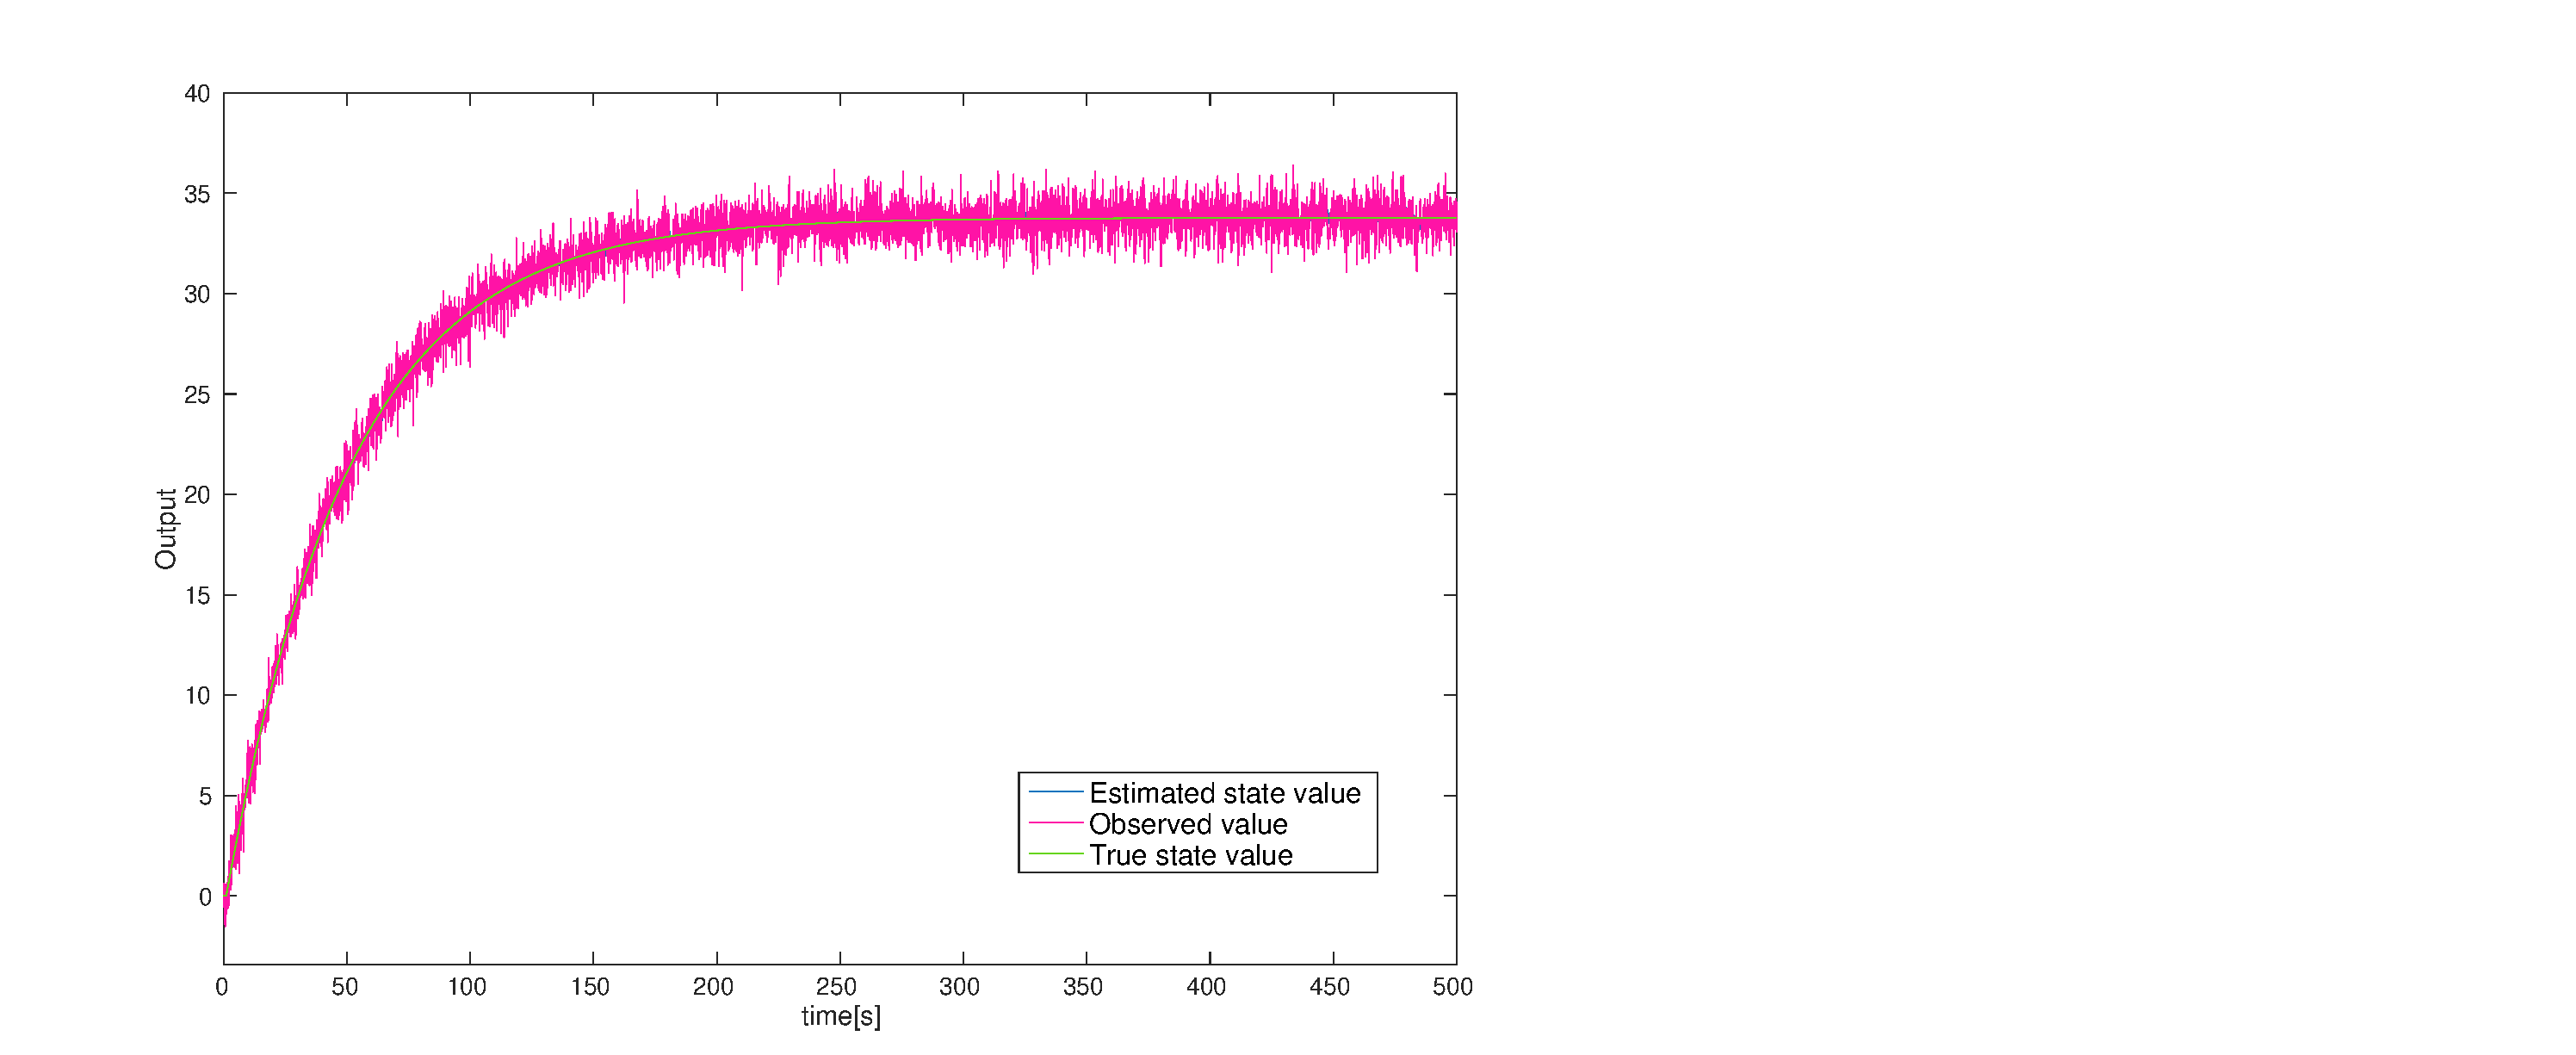
\includegraphics[scale=0.52]{../figure/eps/alloutput.eps}\\
 \hspace{0.0cm}
 (a) すべての出力\\
 \vspace{1.2cm}
 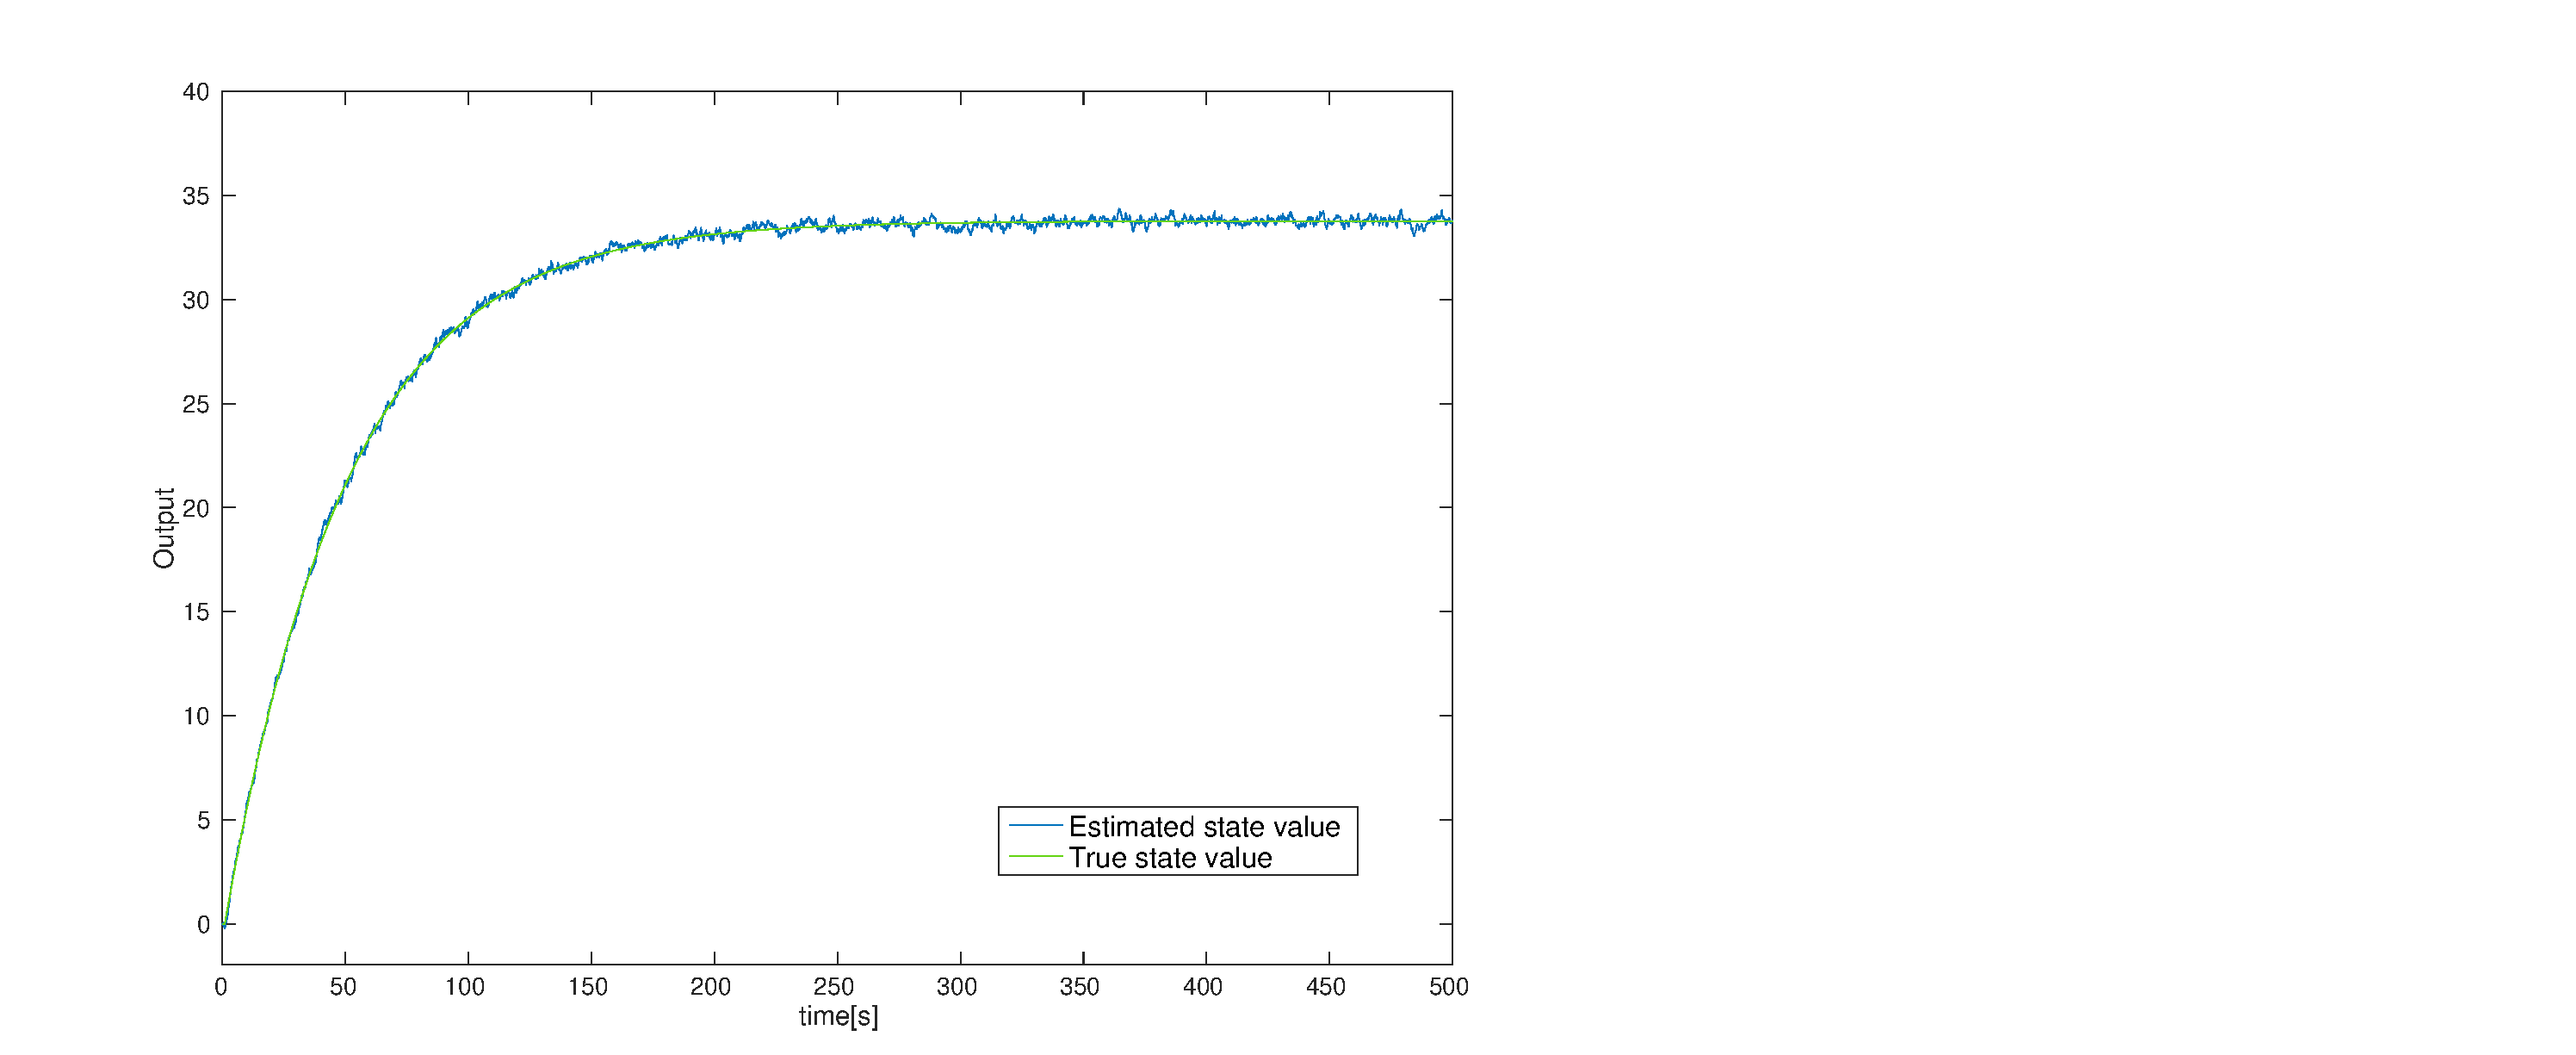
\includegraphics[scale=0.52]{../figure/eps/estimated.eps}\\
 (b) 真値と推定値の比較\\
 \caption{シミュレーション結果}
 \label{result}
\end{figure}


\newpage
% 参考文献
\begin{thebibliography}{99}
\addcontentsline{toc}{section}{参考文献}
\bibitem{2} 足立 修一,丸田 一郎,”カルマンフィルタの基礎”,東京電機大学出版局,pp.8-13,122-134,2013.
\bibitem{3} 加藤 寛一郎,”最適制御入門”,東京大学出版会,pp.129-140,1996.
\bibitem{4} 有本 有,”カルマン・フィルター”,産業図書株式会社,pp.89-139,1994.
\bibitem{5} 片山 徹,”新版 応用カルマンフィルタ”,朝倉書店,pp.108-123,2002.
\bibitem{1} T.Sakamoto,”Lecture Note of Advanced Electrical Drive Control System”,pp.44-46,2017.
\end{thebibliography}

\end{document}
